
\section{Inciso 1}

El proceso es claramente adiabático y se tiene, mediante un ajuste realizado
   con \textit{GNUPLOT}, que el coeficiente $\gamma = 1.309$, el cual es muy aproximado al
   $\flatfrac{7}{5}$. En la gráfica "\textit{ajuste.pdf}" se puede ver la relación entre el ajuste
   y los datos. (programa "\textit{ajuste.gp}")
   
\begin{figure}[h]
	   \centering
	   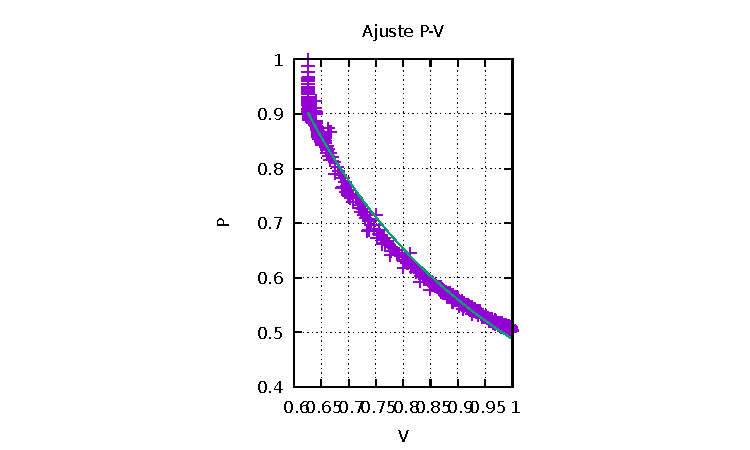
\includegraphics[scale=1.2]{ajuste.pdf}
	   \caption{Ajuste realizado con los datos proporcionados mediante el lenguaje GNUPLOT y la función \textit{fit}.}
	   \label{inciso1}
\end{figure}

\section{Inciso 2}

En $1.6 min$, dada la gráfica "\textit{inciso2.pdf}", es claro que la temperatura
   se mantiene constante en el intervalo mostradp. (programa "\textit{graph.py}")

\begin{figure}[H]
	\centering
	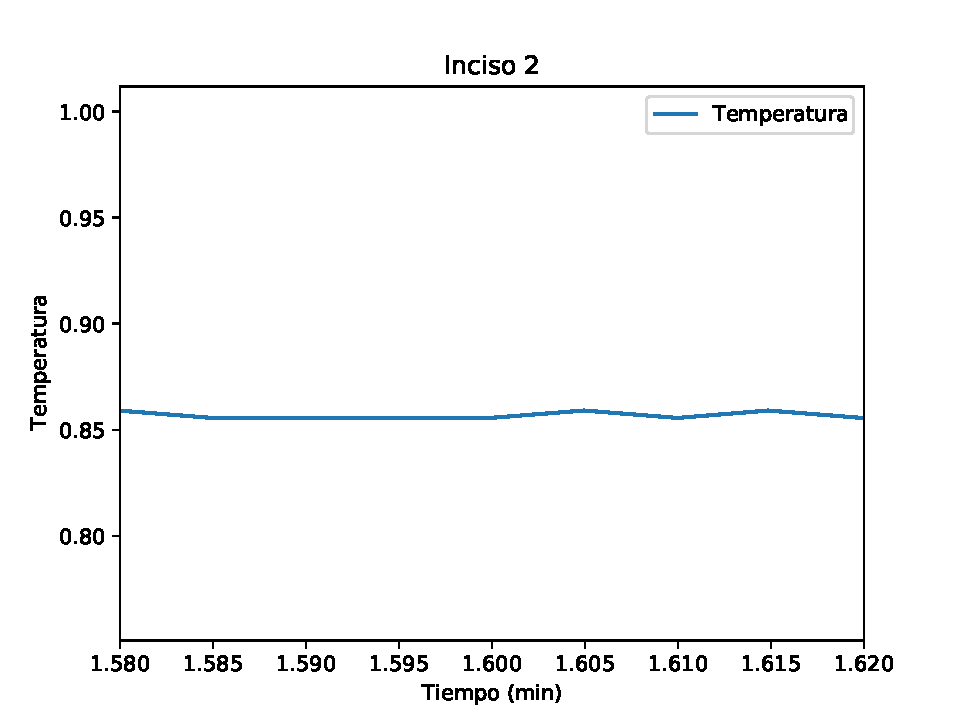
\includegraphics[scale=0.8]{inciso2.pdf}
	\caption{Gráfica Termperatura vs Tiempo que muestra un proceso isotérmico.}
\end{figure}





























